\section{Environments, scoping and parameter passing}
\label{sec:scoping}

This section follows Scott and Aldrich~\cite[Ch.~3]{scott2025pragmatics},
Friedman and Wand~\cite[Sec.~3.5--3.7]{friedman2008essentials},
Lee~\cite[Sec.~5.9]{lee2017foundations} and Aho et
al.~\cite[Sec.~1.6]{aho2007compilers}.

\subsection{Variables and bindings}

Variables appear in a program as declarations or as references. A
\textbf{declaration} introduces a variable into the program and makes it
available at run time; a \textbf{reference} is a use of the variable. The
lecture's declarations come from many languages: \texttt{val imAVar = 3},
\texttt{int myVar;}, \texttt{(defvar x 42)}, \texttt{let var = "string";},
\texttt{variable\_name = 2.71}, \texttt{var aVar string = "variable"},
\texttt{AVar2 := "new declaration"} and the parameter of
\texttt{(lambda (x) x)}. A variable is bound by the declaration that declares
it, and through it to its value.

\subsection{Scopes}

\begin{definition}
The \textbf{scope} of a declaration is the part of the program where the
variable is valid and visible.
\end{definition}

Scopes manage declarations (as symbol tables do) and let the same name be
reused without undesired side effects. In
\codelines{Scheme}{scheme/scoping.scm}{7}{12}
the outer \texttt{let} creates a scope with $x = 3$ and $y = 4$, the inner one a
scope with $x = y + 5 = 9$, and each application of \texttt{*} and \texttt{+}
runs in a scope of its own. Figure~\ref{fig:let-envs} shows the environments
when \texttt{(* x y)} runs: \texttt{x} is found in the inner environment and
\texttt{y} in the outer one. The product is 36, and the outer sum adds the
outer \texttt{x}: the result is 39.

\begin{figure}[h]
\centering
\begin{tikzpicture}[env/.style={draw, rounded corners=2pt, align=left, font=\small\ttfamily, inner sep=4pt}]
  \node[env] (outer) at (0,0) {x $\mapsto$ 3\\y $\mapsto$ 4};
  \node[env] (inner) at (4,0) {x $\mapsto$ 9};
  \node[env] (mul) at (8,0) {r $\mapsto$ 36};
  \draw[flecha] (inner) -- node[above, font=\footnotesize] {parent} (outer);
  \draw[flecha] (mul) -- node[above, font=\footnotesize] {parent} (inner);
  \node[font=\footnotesize, below=2mm of outer] {outer \texttt{let}};
  \node[font=\footnotesize, below=2mm of inner] {inner \texttt{let}};
  \node[font=\footnotesize, below=2mm of mul] {result of \texttt{(* x y)}};
\end{tikzpicture}
\caption{Environments while evaluating \texttt{(* x y)}.}
\label{fig:let-envs}
\end{figure}

Each scope creates an environment for the execution of the program, with
its rules of validity and visibility. The lecture compares three rules. With
static scoping, a name is bound by the closest declaration in the text,
moving outward. With dynamic scoping, it is bound according to where the
function is called, so different calls may give different results. Qualified
names group names under a prefix to avoid collisions between scopes.

\subsection{Static scoping}

\begin{definition}
The \textbf{static (lexical) scoping} rule: to find the declaration of a use
of a variable, search outward from the scope of the use, through the
enclosing scopes, until a declaration is found. Variables that follow this
rule are \textbf{lexical variables}.
\end{definition}

Scopes are delimited by code blocks (\texttt{\{\dots\}}): blocks, function
definitions, control statements and objects each create a scope nested in
the scope where they are declared, with its own memory space. Function
definitions create a scope in which each parameter is a variable, plus the
variables of the body. A function runs in the scope where it was defined:
its free variables are bound by the declarations around its definition, not
around its call.
\codelines{Scheme}{scheme/scoping.scm}{15}{19}
\texttt{(g)} returns 10: the \texttt{x} in the body of \texttt{f} is the global
one, the declaration around the definition of \texttt{f}, even though \texttt{f}
is called from inside the \texttt{let} of \texttt{g}.

\paragraph{Holes and shadows.} A declaration in an inner scope with the same
name as an outer one \textbf{shadows} it: inside the inner scope the outer
variable is not visible, and the region where it is hidden is a hole in its
scope.
\codelines{C++}{cpp/scoping.cpp}{9}{23}
The program prints \texttt{3 2}, \texttt{1 4}, \texttt{1 2} and \texttt{1 1}
(Figure~\ref{fig:shadows}). In the first inner block, \texttt{a = 3} shadows
the outer \texttt{a} and \texttt{b = 2} is visible from the enclosing block.
In the second, \texttt{b = 4} shadows \texttt{b = 2} and the outer \texttt{a} is
visible. After the blocks, each name refers to its outer declaration again.

\begin{figure}[h]
\centering
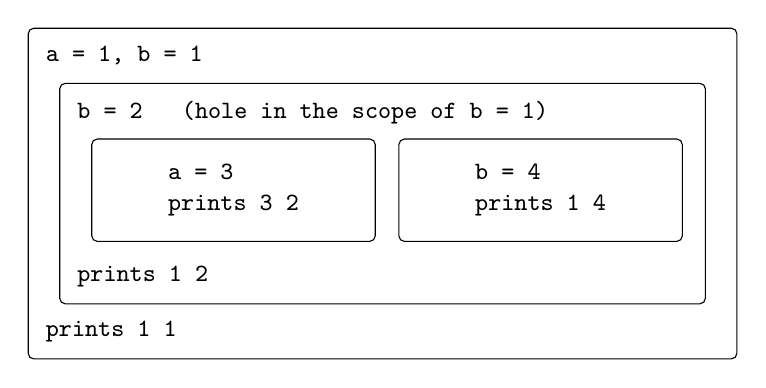
\begin{tikzpicture}[blk/.style={draw, rounded corners=2pt, font=\small\ttfamily, align=left, inner sep=4pt, anchor=north west}]
  \draw[rounded corners=2pt] (0,0) rectangle (9,-4.2);
  \node[anchor=north west, font=\small\ttfamily] at (0.1,-0.1) {a = 1, b = 1};
  \draw[rounded corners=2pt] (0.4,-0.7) rectangle (8.6,-3.5);
  \node[anchor=north west, font=\small\ttfamily] at (0.5,-0.8) {b = 2 \quad (hole in the scope of b = 1)};
  \node[blk, minimum width=3.6cm, minimum height=1.3cm] at (0.8,-1.4) {a = 3\\prints 3 2};
  \node[blk, minimum width=3.6cm, minimum height=1.3cm] at (4.7,-1.4) {b = 4\\prints 1 4};
  \node[anchor=north west, font=\small\ttfamily] at (0.5,-2.9) {prints 1 2};
  \node[anchor=north west, font=\small\ttfamily] at (0.1,-3.6) {prints 1 1};
\end{tikzpicture}
\caption{Nested blocks of the shadowing example and what each \texttt{cout} prints.}
\label{fig:shadows}
\end{figure}

\paragraph{Extent.} The \textbf{extent} of a binding is the time during which
it is valid. Bindings are usually valid while the block that defines them
runs, but they can live longer, even indefinitely, when a closure that
refers to them is returned:
\codelines{Scheme}{scheme/scoping.scm}{22}{26}
\texttt{count} belongs to a call of \texttt{make-counter} that has finished,
but the returned function still uses it. Scope is a property of the text;
extent is a property of the execution.

\paragraph{Lexical depth.} As with symbol tables, each new block has its own
environment with a link to its parent. In \texttt{let x = exp1 in let y = exp2
in -(x, y)}, the environment of the body has $y$ at depth 0 and $x$ at depth 1
(Figure~\ref{fig:depth}). Because scoping is static, the depth of each use is
known before the program runs, and a compiler can replace each name with a
pair (depth, position): a lexical address.

\begin{figure}[h]
\centering
\begin{tikzpicture}[env/.style={draw, rounded corners=2pt, font=\small, inner sep=4pt}]
  \node[env] (e0) at (0,0) {empty};
  \node[env] (e1) at (3.5,0) {$x \mapsto \mathit{val}_1$};
  \node[env] (e2) at (7,0) {$y \mapsto \mathit{val}_2$};
  \draw[flecha] (e1) -- (e0);
  \draw[flecha] (e2) -- (e1);
  \node[font=\footnotesize, below=2mm of e2] {depth 0 for the body};
  \node[font=\footnotesize, below=2mm of e1] {depth 1};
  \node[font=\small] at (7,1) {\texttt{-(x, y)}: $x$ at (1, 0), $y$ at (0, 0)};
\end{tikzpicture}
\caption{Environments and lexical depth for \texttt{let x = exp1 in let y = exp2 in -(x, y)}.}
\label{fig:depth}
\end{figure}

Summing up the rule: variables get their meaning from their location in the
code. Look for the variable in the current environment; if it is found, use
it; if not, go to the next enclosing scope and repeat. Operations with
lexical scope always do the same thing, wherever they are called.

\subsection{Dynamic scoping}

\begin{definition}
The \textbf{dynamic scoping} rule: the value of a variable is the one of the
most recently called procedure that is still active and declares the
variable.
\end{definition}

The lecture shows the difference in Perl:
\codelines{Perl}{perl/dynamic.pl}{4}{6}
With static scoping, the \texttt{\$x} of \texttt{f} is the global one and
\texttt{g()} returns 10. With dynamic scoping, when \texttt{f} runs the most
recent active function that declares \texttt{\$x} is \texttt{g}, so \texttt{g()}
returns 20; Perl's \texttt{local} gives exactly this behavior, and the test
checks that \texttt{g()} is 20 and \texttt{f()} alone is 10. In Common Lisp,
variables declared with \texttt{defvar} are dynamically scoped (special), and
the same program reads:
\codelines{CommonLisp}{lisp/dynamic.lisp}{5}{11}
A variable bound with \texttt{let} that was not declared special is lexical:
\codelines{CommonLisp}{lisp/dynamic.lisp}{16}{22}
\texttt{(g-lex)} returns 10. Shell variables are also dynamic:
\codelines{bash}{bash/dynamic.sh}{1}{3}

The lecture's second Perl example adds \texttt{sub h(param) \{ local \$x = param
+ 5; return f(); \}} and calls \texttt{h(rand(100))} from \texttt{g}: now
\texttt{f} sees the \texttt{\$x} of \texttt{h}, which is different in every call.
The behavior of an operation with dynamic scope can change with every call.

\paragraph{Logo.} The third example is in Logo, which uses dynamic scoping. A
procedure \texttt{test1} with parameter \texttt{:x} only calls \texttt{test2};
\texttt{test2} prints \texttt{In test2:} followed by \texttt{:x}. The program
sets the global \texttt{x} to \texttt{"foo} and calls \texttt{test1 "bar}.
\texttt{test2} called alone prints \texttt{foo}, the global value. Called from
\texttt{test1 "bar}, it prints \texttt{bar}: the most recent active procedure
with \texttt{x} is \texttt{test1}, whose parameter \texttt{x} is \texttt{"bar}.
\codelines{CommonLisp}{lisp/dynamic.lisp}{26}{28}

\paragraph{Advantages and disadvantages.} Dynamic scoping favors flexibility:
variables can be accessed from anywhere, which can help reuse and adaptation
of code. It is harder to reason about, the flow is harder to understand, it
can be slower (no static optimizations such as lexical addresses), and it is
error-prone because of unintended accesses to variables.

\subsection{Qualified names and access modifiers}

Global variables can be accessed from the whole program, which causes name
collisions. With \textbf{qualified names}, related names are grouped under a
name, the prefix, and a variable has two sets of scopes: a scope (usually the
global one) where the qualified name \texttt{Group.name} is visible, and one or
more narrower scopes where the unqualified name is visible as well. Modules,
packages and namespaces work this way.

\textbf{Access modifiers} restrict visibility further, beyond the scoping rules.
A private member is only visible inside the object (it is part of the
implementation); a public member is visible anywhere (it is part of the
interface). The details depend on the language; Table~\ref{tab:access} shows
Swift's levels.

\begin{table}[h]
\centering
\small
\begin{tabular}{l c c c c}
  \toprule
  Modifier & Immediate scope & File & Containing module & Rest of the world \\
  \midrule
  \texttt{open}, \texttt{public} & yes & yes & yes & yes \\
  \texttt{internal}               & yes & yes & yes & no \\
  \texttt{fileprivate}            & yes & yes & no  & no \\
  \texttt{private}                & yes & no  & no  & no \\
  \bottomrule
\end{tabular}
\caption{Where a declaration is visible for each access modifier in Swift. \texttt{open} also allows subclassing outside the module.}
\label{tab:access}
\end{table}

\subsection{Environments and stores}

This subsection goes beyond the slides. An \textbf{environment}
$\rho : \mathit{Var} \to \mathit{Loc}$ maps names to locations, and a \textbf{store}
$\sigma : \mathit{Loc} \to \mathit{Val}$ maps locations to values; reading $x$ is
$\sigma(\rho(x))$. SIMP used a single map, $\mathit{Var} \to \mathit{Val}$, but separating
the two is what allows two names to refer to the same location (a reference
parameter, a closure) and one name to refer to different locations at
different times (a recursive call, a shadowing declaration). The parameter
passing modes below are differences in how $\rho$ and $\sigma$ are extended.

\paragraph{Closures in loops.} A closure captures a binding, not a value. In
Python a loop has one variable for all its iterations; JavaScript's
\texttt{let} creates a new one in each iteration:
\codelines{Python}{python/loopvar.py}{1}{7}
\codelines{JavaScript}{js/loopvar.js}{2}{9}

\subsection{Parameter passing}

The parameters written in a call are the \textbf{actual} parameters; the
parameters in the definition of the function are the \textbf{formal}
parameters. The modes differ in what the formal parameter is bound to.

\paragraph{Call by value.} The actual parameters are evaluated, and their
values copied into the space of the formal parameters (the space of the
function). Changes to the formal parameters do not affect the caller.

\paragraph{Call by reference.} The address of the actual parameter is passed,
and the function uses it directly. The formal parameter is another name for
the caller's variable.
\codelines{C++}{cpp/scoping.cpp}{27}{28}
In the lecture's program, \texttt{swap(x, y)} with $x = 1$, $y = 2$ prints
\texttt{After Swapping in function x: 2, y: 1} in both cases, but
\texttt{main} prints \texttt{x: 1, y: 2} with call by value and
\texttt{x: 2, y: 1} with call by reference.

\paragraph{Call by name.} Call by name is between values and references: the
function sees the parameter as if it were a copy, but the argument expression
is never evaluated at the call; it is evaluated, in the caller's environment,
each time the parameter is used (with variables renamed if needed). With
\texttt{int x = 1, y = 2+8;} and \texttt{swap(x, y)} by name, \texttt{t = x} reads
1, \texttt{x = y} evaluates the expression of \texttt{y} and writes 10,
\texttt{y = t} writes 1: the program prints \texttt{x: 10, y: 1}. In Scheme the
names can be passed as functions that read and write the caller's variables:
\codelines{Scheme}{scheme/scoping.scm}{33}{42}

\paragraph{Passing parameters between procedures.} The lecture compares the
modes with one program:
\begin{lstlisting}
Program Test
  Var x: int, y: int; v[5]: int;
  Proc p1(val a: int, ref b: int, ref c: int)
  Begin
    b = b + 1;
    c = a;
  end
Begin
  v = [0,1,2,3,4]
  x = 10;
  y = 1
  p1(x, y, v[y]);
end
\end{lstlisting}
and then changes the mode of \texttt{b} and \texttt{c}. Table~\ref{tab:params}
gives the result of each version.

\begin{table}[h]
\centering
\small
\begin{tabular}{l l >{\raggedright\arraybackslash}p{0.3\textwidth} >{\raggedright\arraybackslash}p{0.24\textwidth}}
  \toprule
  Modes of $a, b, c$ & $b = b + 1$ & $c = a$ & At the end \\
  \midrule
  val, ref, ref   & $y = 2$ & $v[1] = 10$ ($c$ was bound to $v[1]$ at the call) & $y = 2$, $v = [0,10,2,3,4]$ \\
  val, ref, name  & $y = 2$ & $v[2] = 10$ ($v[y]$ is evaluated now, with $y = 2$) & $y = 2$, $v = [0,1,10,3,4]$ \\
  val, VR, name   & local $b = 2$ & $v[1] = 10$ ($y$ is still 1) & $y = 2$ (copied back), $v = [0,10,2,3,4]$ \\
  \bottomrule
\end{tabular}
\caption{The program \texttt{Test} with three combinations of modes. $a$ is always $x = 10$.}
\label{tab:params}
\end{table}

\textbf{Value-result} (copy-restore, VR) copies the value in at the call, works on
a local copy and copies it back at the return. With \texttt{b} by value-result
the change to $y$ is not visible during the call, so \texttt{v[y]} still means
\texttt{v[1]}. In C++ a reference parameter is \texttt{int\&}, a parameter by
name can be a function that returns a reference, and value-result is a copy
made by hand:
\codelines{C++}{cpp/scoping.cpp}{30}{39}

\paragraph{Other kinds.} The lecture also lists call by move (Emerald),
adaptive parameter passing, streaming semantics, cache semantics and lazy
semantics or call by need. Call by need is call by name where the argument is
evaluated at most once and the value is remembered; the runtime block
studies it.

\subsection{A small-step rule for calls}

This subsection goes beyond the slides. A procedure value is a closure
$\mathbf{proc}(x, C, \rho_{\mathit{def}})$: the parameter, the body and the
environment where the procedure was defined. Call by value allocates a new
location for the parameter:
\begin{mathpar}
\inferrule*[right=Call-By-Value]
  {\sigma(\rho(f)) = \mathbf{proc}(x, C, \rho_{\mathit{def}}) \\
   \langle E, \rho, \sigma \rangle \Downarrow v \\
   \ell \notin \mathrm{dom}(\sigma) \\
   \langle C, \rho_{\mathit{def}}[x \mapsto \ell], \sigma[\ell \mapsto v] \rangle \Downarrow \sigma''}
  {\langle \mathbf{call}\ f(E), \rho, \sigma \rangle \to \langle \mathtt{skip}, \rho, \sigma'' \rangle}
\end{mathpar}
The argument is evaluated in the caller's environment $\rho$, and the body
runs in the closure's environment $\rho_{\mathit{def}}$: that is static scoping.
With dynamic scoping the body would run in $\rho[x \mapsto \ell]$, the caller's
environment. Call by reference binds $x$ to the existing location of the
argument instead of a new one: $\rho_{\mathit{def}}[x \mapsto \rho(y)]$.

\subsection{Exercises}

\begin{exercise}
Give the values of the variables in each step of
\texttt{(let ((x 3) (y 4)) (+ (let ((x (+ y 5))) (* x y)) x))}.
\end{exercise}

\paragraph{Solution.} The outer \texttt{let} binds $x = 3$, $y = 4$. The inner one
evaluates \texttt{(+ y 5)} in the outer environment, 9, and binds $x = 9$. The
product reads $x = 9$ (inner) and $y = 4$ (outer): 36. Back in the outer scope,
the sum reads $x = 3$: $36 + 3 = 39$.

\begin{exercise}
What does the shadowing program print if the declaration \texttt{int b = 2;}
is replaced by the assignment \texttt{b = 2;}?
\end{exercise}

\paragraph{Solution.} Now there is only one \texttt{b}, and the assignment changes
it. The prints are \texttt{3 2}, \texttt{1 4}, \texttt{1 2} and, at the end,
\texttt{1 2}: the last line sees the \texttt{b} that was assigned 2.

\begin{exercise}
With dynamic scoping, what does \texttt{g()} return in the Perl example if
\texttt{g} calls \texttt{h(7)} and \texttt{h} calls \texttt{f}?
\end{exercise}

\paragraph{Solution.} When \texttt{f} runs, the active procedures are \texttt{g}
(with \texttt{\$x = 20}) and \texttt{h} (with \texttt{\$x = 7 + 5 = 12}). The most
recent is \texttt{h}, so the result is 12. With static scoping it would be 10.

\begin{exercise}
Run \texttt{test(i, a[i], i)} with $a = [0, 10, 20, 40]$, $i = 0$, and
\texttt{proc test(ref x, name y, VR z) \{ x := x + 1; y := y + 1; z := z + 2;
y := y + 1 \}}.
\end{exercise}

\paragraph{Solution.} $x$ is another name for $i$, $y$ re-evaluates \texttt{a[i]} at
each use, and $z$ starts as a local copy of $i$, 0. \texttt{x := x + 1} makes
$i = 1$. \texttt{y := y + 1} evaluates \texttt{a[i]} with $i = 1$: $a[1] = 11$.
\texttt{z := z + 2} gives $z = 2$, locally. The second \texttt{y := y + 1} again
uses $a[1]$: 12. At the return, value-result copies $z$ back into $i$: $i = 2$,
which overwrites the change made through $x$. The final state is $i = 2$,
$a = [0, 12, 20, 40]$.
